% 	Name		:: 	sthlm Beamer Theme  HEAVILY based on the hsrmbeamer theme (Benjamin Weiss)
%	Author		:: 	Mark Hendry Olson (mark@hendryolson.com)
%	Created		::	2013-07-31
%	Updated		::	June 18, 2015 at 08:45
%	Version		:: 	1.0.2
%	Email		:: 	hendryolson@gmail.com
%	Website		:: 	http://v42.com
%
% 	License		:: 	This file may be distributed and/or modified under the
%                  	GNU Public License.
%
%	Description	::	This presentation is a demonstration of the sthlm beamer
%					theme, which is HEAVILY based on the HSRM beamer theme created by Benjamin Weiss
%					(benjamin.weiss@student.hs-rm.de), which can be found on GitHub
%					<https://github.com/hsrmbeamertheme/hsrmbeamertheme>.


%-=-=-=-=-=-=-=-=-=-=-=-=-=-=-=-=-=-=-=-=-=-=-=-=
%
%        LOADING DOCUMENT
%
%-=-=-=-=-=-=-=-=-=-=-=-=-=-=-=-=-=-=-=-=-=-=-=-=

\documentclass[newPxFont]{beamer}
\usetheme{sthlm}
%\usecolortheme{sthlmv42}
\setbeamertemplate{caption}[numbered]

%-=-=-=-=-=-=-=-=-=-=-=-=-=-=-=-=-=-=-=-=-=-=-=-=
%        LOADING PACKAGES
%-=-=-=-=-=-=-=-=-=-=-=-=-=-=-=-=-=-=-=-=-=-=-=-=
\usepackage[utf8]{inputenc}
\usepackage{caption}
\usepackage{chronology}

\renewcommand{\event}[3][e]{%
  \pgfmathsetlength\xstop{(#2-\theyearstart)*\unit}%
  \ifx #1e%
    \draw[fill=black,draw=none,opacity=0.5]%
      (\xstop, 0) circle (.2\unit)%
      node[opacity=1,rotate=45,right=.2\unit] {#3};%
  \else%
    \pgfmathsetlength\xstart{(#1-\theyearstart)*\unit}%
    \draw[fill=black,draw=none,opacity=0.5,rounded corners=.1\unit]%
      (\xstart,-.1\unit) rectangle%
      node[opacity=1,rotate=45,right=.2\unit] {#3} (\xstop,.1\unit);%
  \fi}%

%-=-=-=-=-=-=-=-=-=-=-=-=-=-=-=-=-=-=-=-=-=-=-=-=
%        BEAMER OPTIONS
%-=-=-=-=-=-=-=-=-=-=-=-=-=-=-=-=-=-=-=-=-=-=-=-=

%\setbeameroption{show notes}

%-=-=-=-=-=-=-=-=-=-=-=-=-=-=-=-=-=-=-=-=-=-=-=-=
%
%	PRESENTATION INFORMATION
%
%-=-=-=-=-=-=-=-=-=-=-=-=-=-=-=-=-=-=-=-=-=-=-=-=

\title{Mobile Big Data Analytics
Using Deep Learning and Apache Spark}
\subtitle{A presentation on research paper based on Deep Learning and Cloud Computing}
\date{}
\author{\texttt{Manash Kumar Mandal, Department of EEE, 2k12}}
\institute{\textit{Khulna University of Engineering \& Technology}}


\begin{document}

%-=-=-=-=-=-=-=-=-=-=-=-=-=-=-=-=-=-=-=-=-=-=-=-=
%
%	TITLE PAGE
%
%-=-=-=-=-=-=-=-=-=-=-=-=-=-=-=-=-=-=-=-=-=-=-=-=

\maketitle

%\begin{frame}[plain]
%	\titlepage
%\end{frame}

%-=-=-=-=-=-=-=-=-=-=-=-=-=-=-=-=-=-=-=-=-=-=-=-=
%
%	TABLE OF CONTENTS: OVERVIEW
%
%-=-=-=-=-=-=-=-=-=-=-=-=-=-=-=-=-=-=-=-=-=-=-=-=


\section*{Overview}
\begin{frame}[allowframebreaks]{Overview}
% For longer presentations use hideallsubsections option
\tableofcontents[hideallsubsections]
\end{frame}

% Definition of Mobile Big Data

\section{What is Mobile Big Data (MBD)?}

\begin{frame}[c]{What is Mobile Big Data (MBD)?}

\alert{Mobile big data (MBD)} is a concept that describes
a massive amount of mobile data that cannot be processed
using a single machine.

\vspace{1em}

\begin{exampleblock}{Application of MBD}
\begin{enumerate}
	\item{Fraud Detection}
    \item{Marketing and Targeted advertising}
    \item{Context-aware computing}
    \item{Health Care}
\end{enumerate}

\end{exampleblock}
\end{frame}

% Concepts and features of MBD

\subsection{Concept and Features of Mobile Big Data (MBD)}

\begin{frame}[c, allowframebreaks]{Concept and Features of MBD}

	\begin{figure}
		\centering
		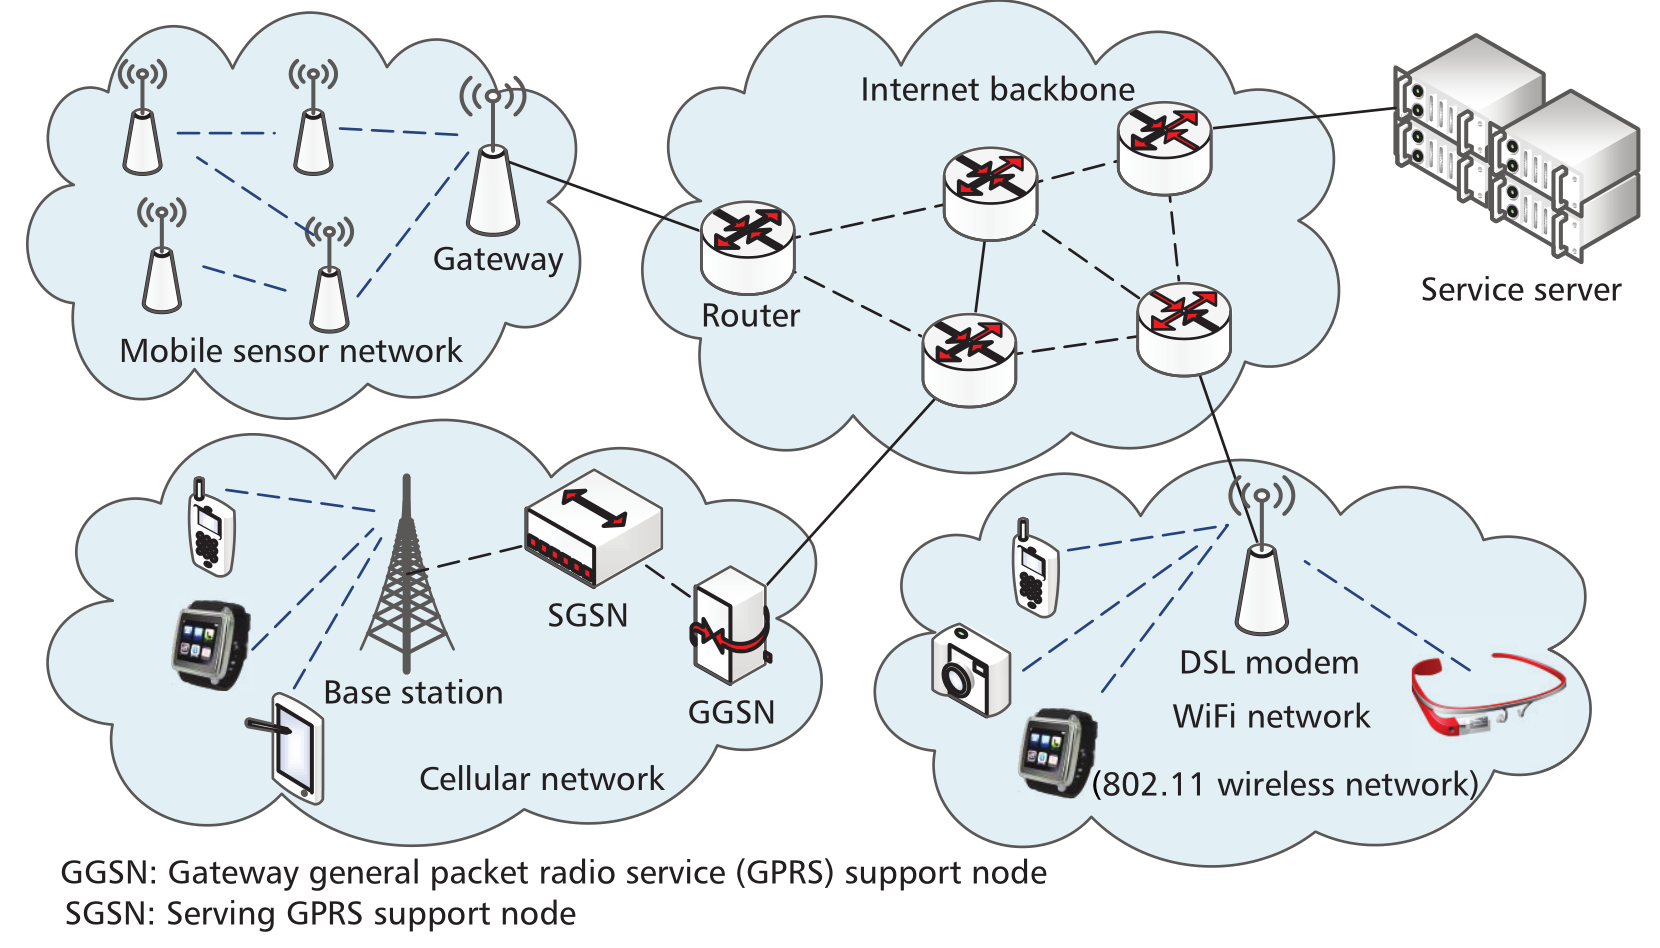
\includegraphics[width=0.9\linewidth]{resources/mbd_architecture.png}
        \captionof{figure}{Typical Architecture of Mobile Network}
        \label{fig:mobileArch}
	\end{figure}
    
    
    \begin{exampleblock}{Concept of MBD}
      \begin{itemize}
          \item{Figure \ref{fig:mobileArch} shows a typical architecture of large-scale mobile
  systems used to connect various types of portable devices.}
          \item{The widespread installation of various types of sensors allows many new applications.}
          \item{Sensory data are stored in JavaScript Object Notation (JSON) structure supported by Android, Tizen, iOS operating systems.}
      \end{itemize}
    \end{exampleblock}
    
    \vspace{3em}
    
    \begin{alertblock}{Features of MBD}
    	\begin{itemize}
        	\item{MBD is massive (volume)}
            \item{MBD is generated at increasing rates (velocity)}
            \item{MBD quality is not guaranteed (veracity)}
            \item{MBD is heterogeneous (variety)}
        \end{itemize}
    \end{alertblock}
    
    \vspace{3em}
    
    \begin{figure}
		\centering
		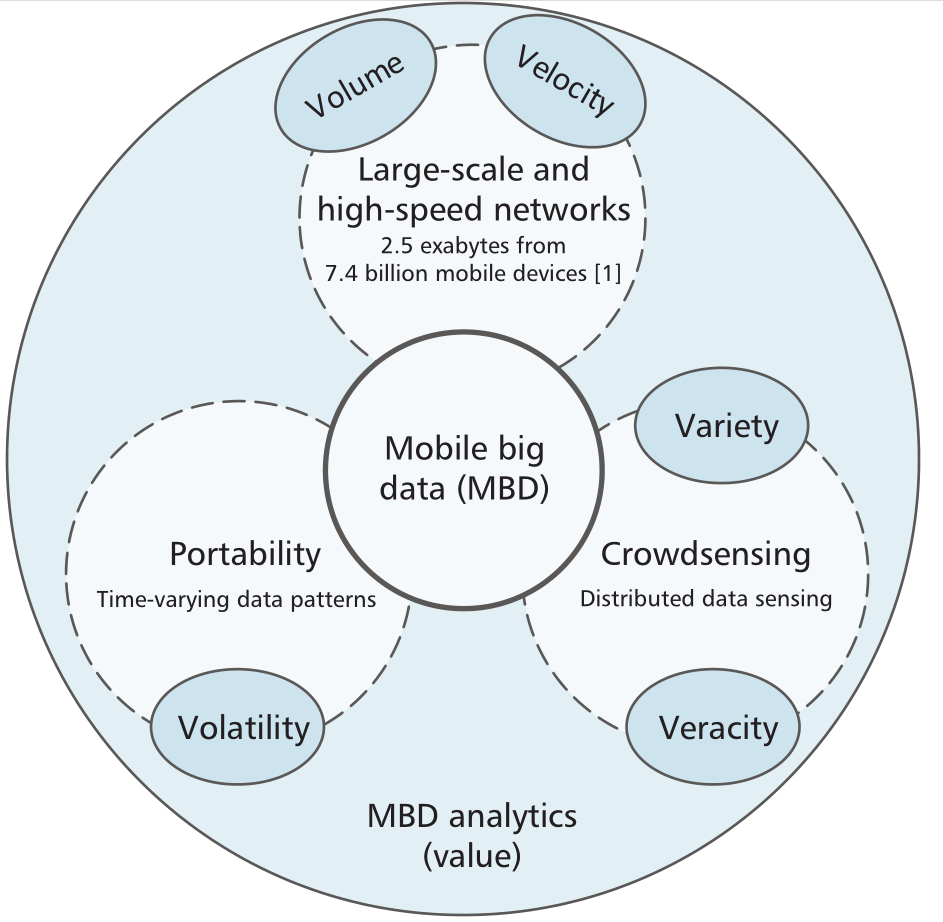
\includegraphics[width=0.6\linewidth]{resources/mbd_structure.png}
        \captionof{figure}{Technological Advances behind Mobile Big Data.}
        \label{fig:mbdEra}
	\end{figure}
    
    \vspace{3em}
 

\end{frame}

\section{Deep Learning}
\begin{frame}[c]{What is Deep Learning?}
\alert{Deep learning} (also known as deep structured learning, hierarchical learning or deep machine learning) is a branch of machine learning based on a set of algorithms that attempt to model high-level abstractions in data by using a deep graph with multiple processing layers, composed of multiple linear and non-linear transformations.

\end{frame}

\subsection{Deep Learning vs Traditional Machine Learning}
\begin{frame}[c]{Deep Learning vs Traditional Machine Learning}

\begin{table}[]
	\begin{tabular}[]{|p{5cm}|p{5cm}|}
		\toprule
		\textbf{Deep Learning}			& \multicolumn{1}{c|}{\textbf{Machine Learning}} \\
		\midrule
		Tries to learn high level features from the given data  & Predicts output from given data			\\[0.25em]
		Deep learning is essentially a set of techniques that helps to parameterize deep neural network structures.
				& 	Traditional machine learning parameterize handful of network parameters	\\[0.25em]
		
		\bottomrule
	\end{tabular}
    \caption{Deep Learning vs Machine Learning}
\end{table}
\end{frame}

% Why are we aiming for deep learning
\begin{frame}[c]{Why we are aiming for Deep Learning}

\begin{exampleblock}{Reasons for Deep Learning}
\begin{itemize}
	\item{Curse of Dimensionality reduction}
    \item{Effective Unsupervised Learning}
    \item{Deep learning can learn from unlabeled data}
    \item{Deep learning generates intrinsic features}
    \item{Multimodal based learning using divide and conquer mechanism}
    \item{Huge reduction in training time}
\end{itemize}
\end{exampleblock}

\end{frame}

\section{Deep learning and MBD}
\subsection{Proposed Deep learning method for MBD Analytics}
\begin{frame}[c, allowframebreaks]{Proposed Deep learning method for MBD analytics}
	\begin{block}{Generative layer-wise pre-training}
    
      \begin{itemize}
			\item{This stage requires only
unlabeled data, which is often abundant and cheap to collect
in mobile systems using crowdsourcing. Figure \ref{fig:training} shows the
layer-wise tuning of a deep model.}

			\item{First one layers pf neurons is trained using the unlabeled data samples. To learn the input data structure, each layer includes encoding and decoding functions.}
            
            \vspace{1em}
            
            \item{The encoding function uses the input data and the layer parameters to generate a set of new features}
            
            
      \end{itemize}
    \end{block}
    
    \vspace{5em}
    
    \begin{figure}
		\centering
		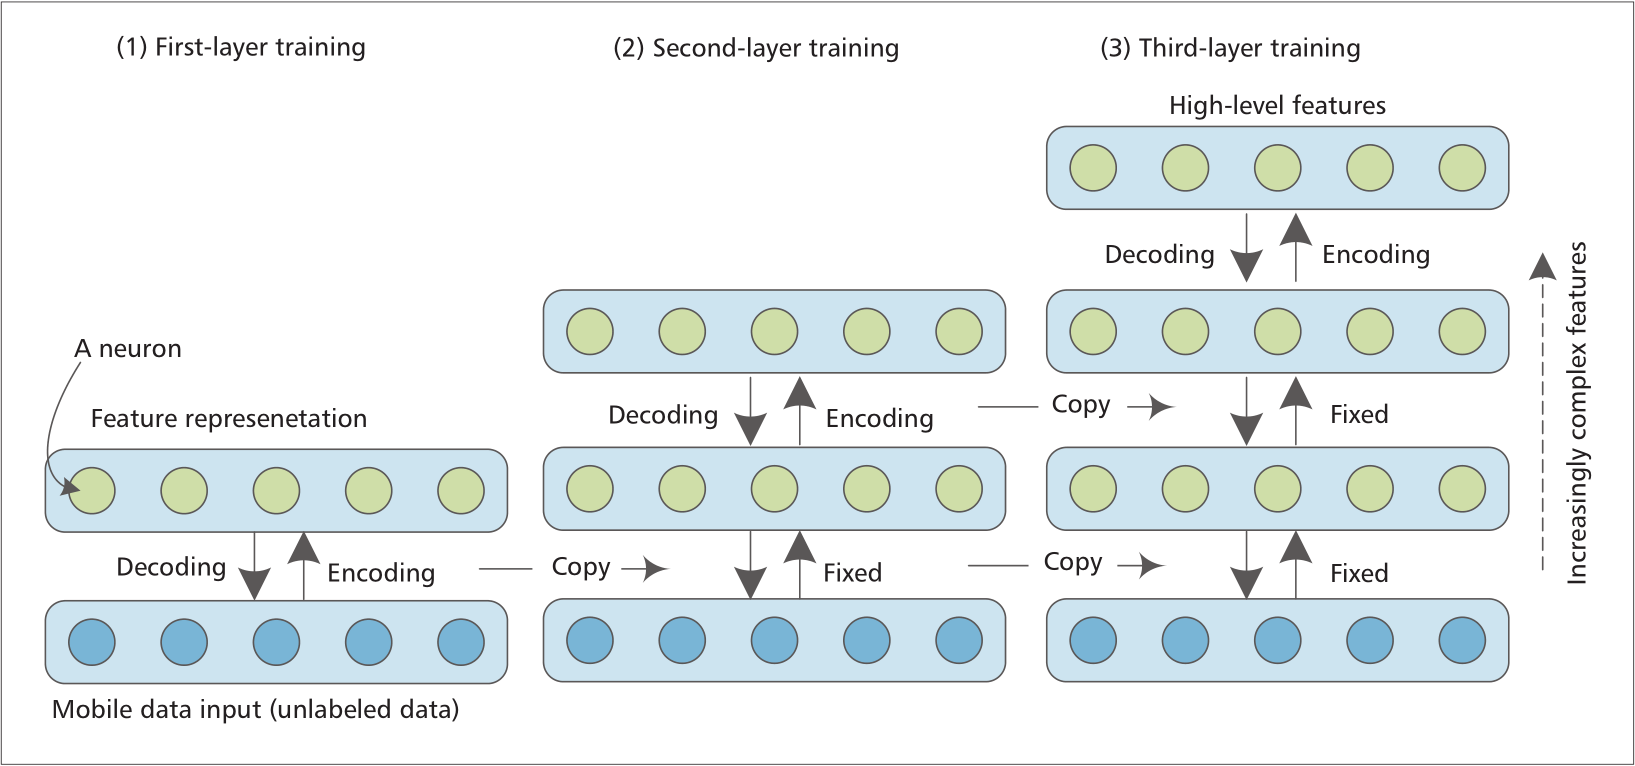
\includegraphics[width=1\linewidth]{resources/deep_learning.png}
        \captionof{figure}{Generative-layer wise training of a deep model}
        \label{fig:training}
	\end{figure}
    
    \vspace{2em}
    
    \begin{block}{Discriminitive fine-tuning}
    	The model’s parameters, which
are initialized in the first step, are then slightly fine-tuned
using the available set of labeled data to solve the problem at
hand.
    \end{block}

\end{frame}

\section{Big Data Processing Framework : Apache Spark}
\subsection{What is Apache Spark}

\begin{frame}[c]{Apache Spark Introduction}
	\begin{alertblock}{What is Apache Spark?}
    	It is a fast and general engine for large-scale data processing.
	\end{alertblock}
    
    \begin{block}{Advantages of using Apache Spark}
    	\begin{itemize}
        	\item{\alert{Speed: } Run programs upto 100x faster than general purpose computers.}
            \item{\alert{Multi Language Support: } Supports various programming languages such as Java, Scala, R and Python.}
            \item{\alert{Long Short Term Memory: } Spark holds intermediate results in memory rather than writing to disk.}
        \end{itemize}
    \end{block}

\end{frame}

\subsection{A Spark-Based Deep Learning Framework for MBD Analytics}
\begin{frame}[allowframebreaks]{Proposed Spark Based Deep Learning Framework}
	\begin{itemize}
		\item{Learning deep models in MBD analytics is slow and computationally demanding.}
        
        \vspace{1em}
        
    	\item{
        	Proposed Spark-based framework consists of two main components:
        	\begin{enumerate}
            	\vspace{0.5em}
            	\item{A Spark Master}
                \vspace{0.5em}
                \item{One or more Spark Workers}
            \end{enumerate}
        }
        
        \vspace{1em}
        
        \item{Figure \ref{fig:proposedFramework} shows architecture of proposed framework.}
    \end{itemize}

\vspace{2em}

	\begin{figure}
		\centering
		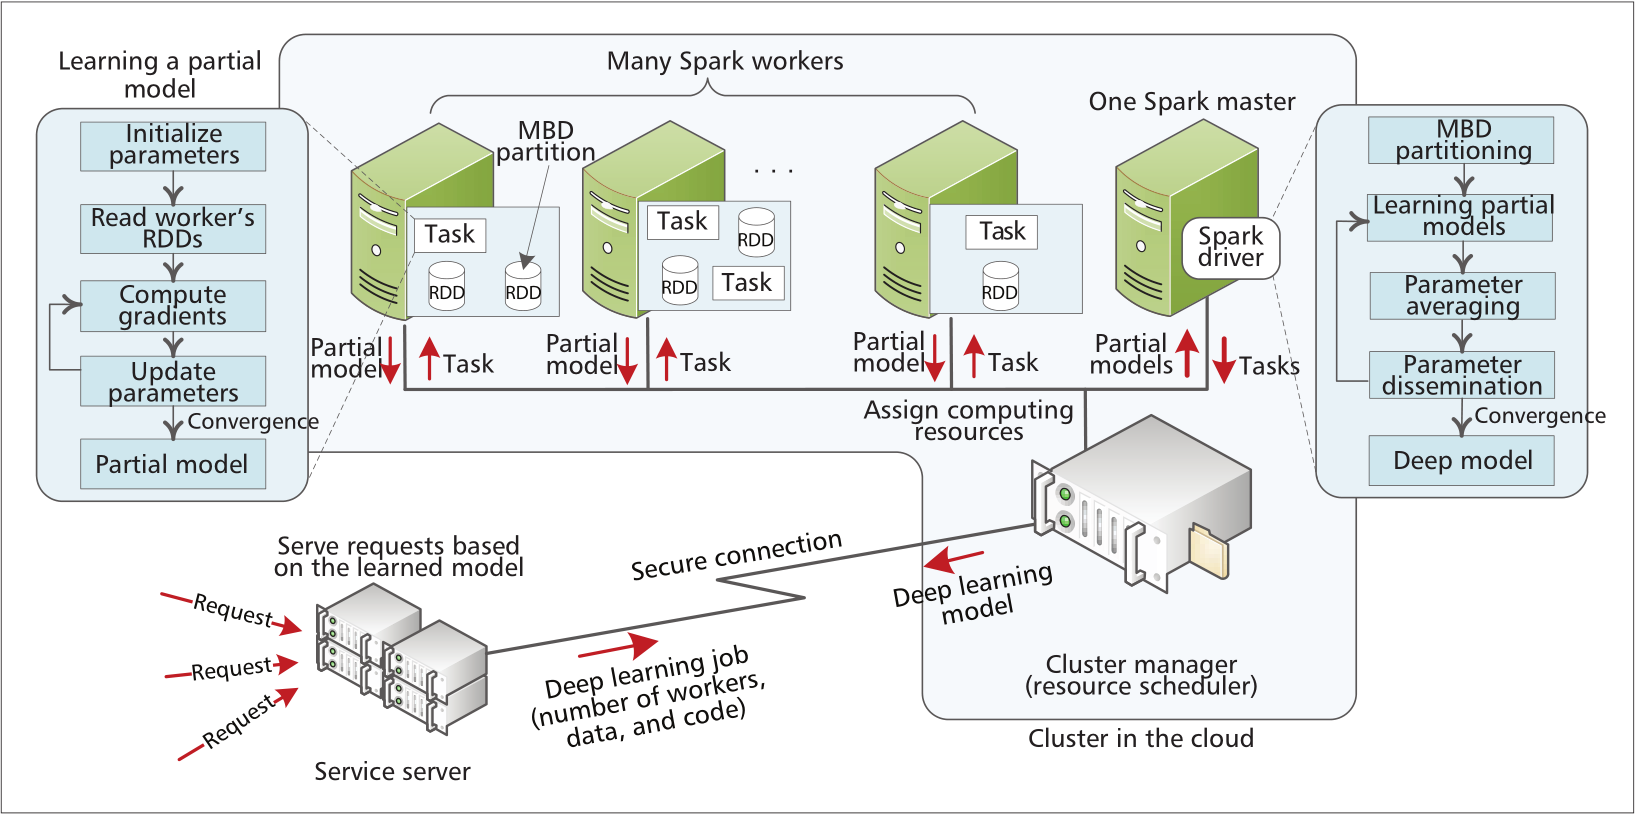
\includegraphics[width=1\linewidth]{resources/sparkmodel.png}
        \captionof{figure}{A Spark-based framework for distributed deep learning in MBD Analytics.}
        \label{fig:proposedFramework}
	\end{figure}

\end{frame}

\subsection{Deep Learning Procedure}
\begin{frame}[allowframebreaks]{Proposed Deep Learning Procedure}
	\begin{block}{Parallelized Learning Collections}
    	Learning deep models can be performed in two main steps:
        	\begin{enumerate}
            	\item{Gradient Computation}
                \item{Parameter Update}
            \end{enumerate}
    \end{block}
    
    \begin{exampleblock}{1. Gradient Computation}
    	Learning Algorithm will iterate through all data batches independently to compute gradient. 
    \end{exampleblock}
    
    \framebreak 
    
    \begin{exampleblock}{2. Parameter Update}
    	In this second step, the model's parameters are updated by averaging the computed gradient updates on all data batches.
    \end{exampleblock}
    
    These two steps fit the learning of deep models in the MapReduce programming model.
 
    \vspace{0.5em}
    
    In particular, the parallel gradient computation is realized as a \textit{Map procedure.}
    
    
\end{frame}

\section{Performance Analysis}
\begin{frame}{Context-Aware Activity Recognition System }
	\begin{block}{Problem Statement}
    	Consider a mobile device with an embedded accelerometer
sensor that generates proper acceleration samples. 

Activity recognition is applied to time series data frames formulated using a sliding and overlapping window.
	
    At time $t$, the activity recognition classifier $f:x_{t}\to S$ matches the framed acceleration data $x_{t}$ with the most probable activity label from the set of supported activity labels $S = \{1, 2, ..., N\}$, where $N$ is the number of supported activities in the activity detection component.
    

    \end{block}
\end{frame}

\subsection{Experimental Analysis and Result}
\begin{frame}[allowframebreaks]{Experimental Analysis using proposed Framework}
	\textit{Activity prediction by Accelerometer's 3-axis signals shown in Fig \ref{fig:activityPrediction}}
    \begin{figure}
		\centering
		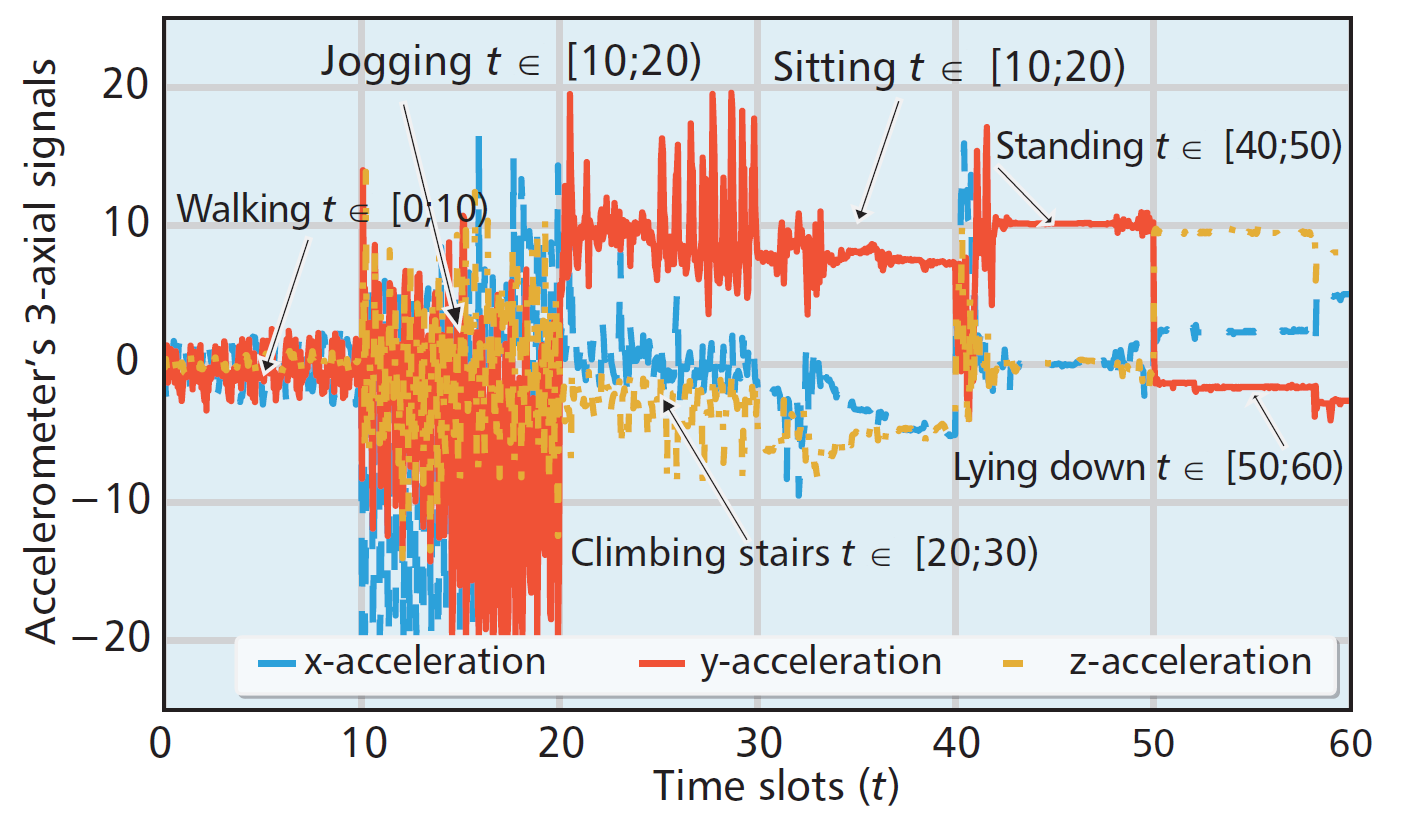
\includegraphics[width=.75\linewidth]{resources/analysis1.png}
        \caption{Accelerometer signal of different human activities.}
        \label{fig:activityPrediction}
	\end{figure}
    
    \framebreak 
    
    \alert{Impact of Deep Models:}
    
    \begin{block}{Relation among Model Construction, 
    Computing Cores and Error}
    
    	\begin{itemize}
			\item{\alert{Model Layer: } Figure \ref{fig:deepModelImpact} shows the activity recognition error under different setups of deep models.}
            \item{\alert{Accuracy Comparison: } Accuracy comparison among different setups can be seen from Figure \ref{fig:deepModelSetupPerformance}}
            \item{\alert{No. of computing Cores: } Speed up efficiency increases drastically with increased number of computing cores. It can be seen from figure \ref{fig:computingCore}}
        \end{itemize}
    \end{block}
    \begin{figure}
		\centering
		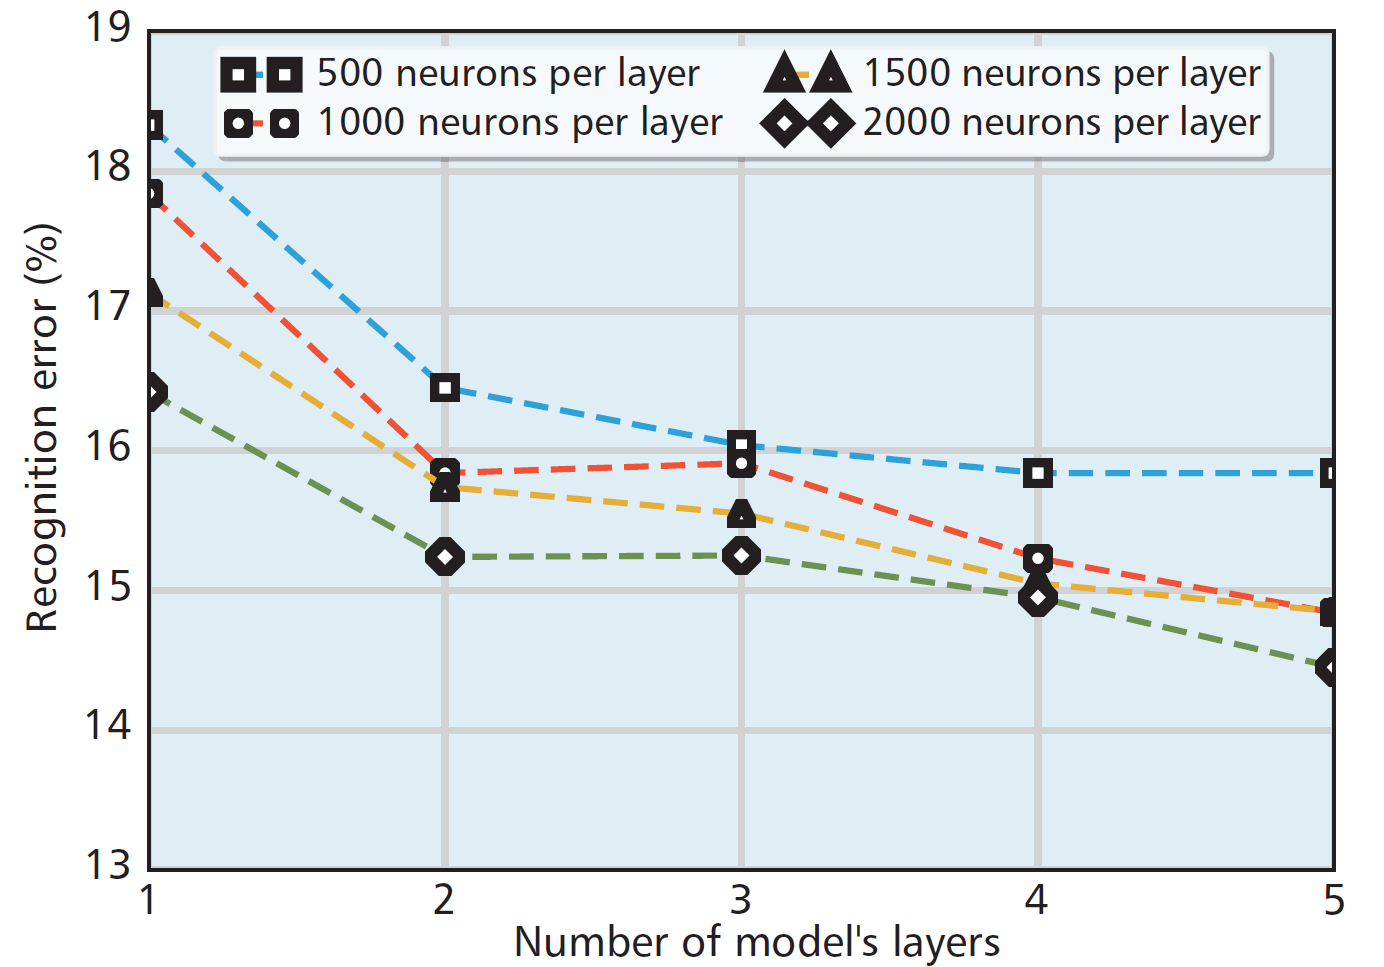
\includegraphics[width=.75\linewidth]{resources/analysis2.png}
        \captionof{figure}{recognition accuracy of deep learning models under different deep model setups.}
        \label{fig:deepModelImpact}
	\end{figure}
    
    \framebreak 
    
    \begin{figure}
		\centering
		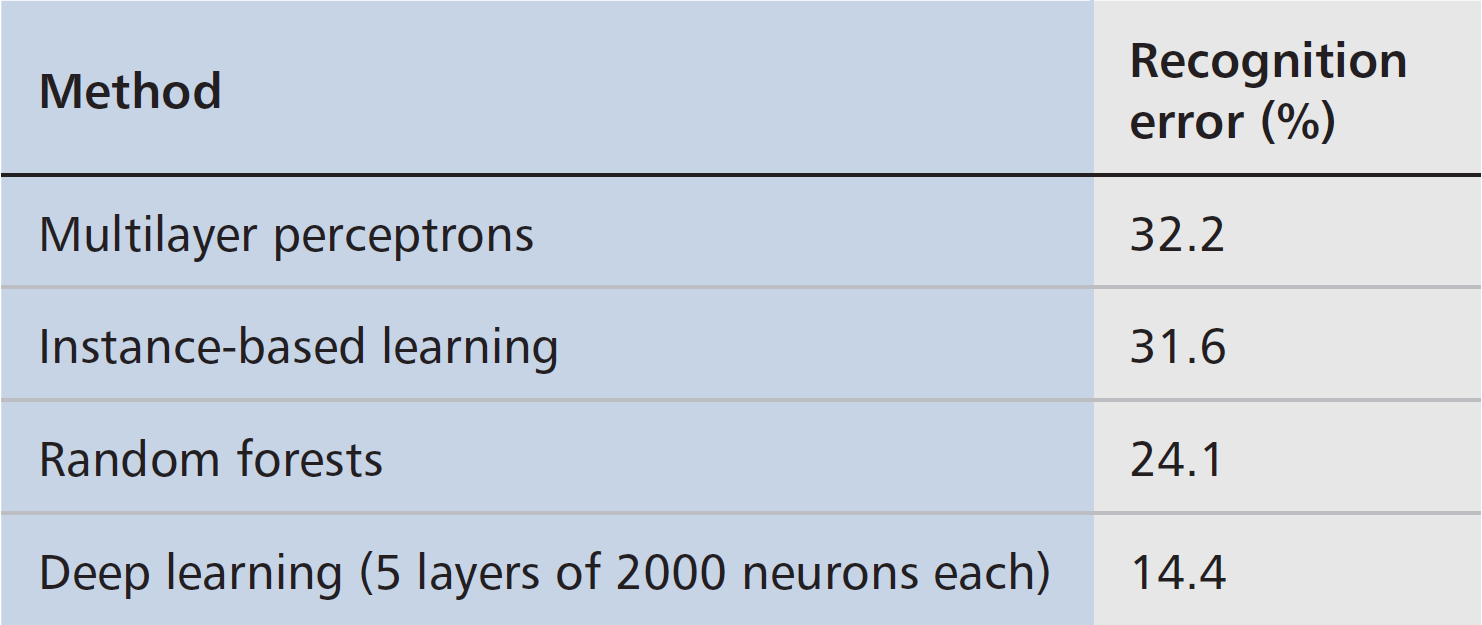
\includegraphics[width=.9\linewidth]{resources/performance2.png}
        \captionof{figure}{Activity recognition error of deep learning and other conventional methods.}
        \label{fig:deepModelSetupPerformance}
	\end{figure}
    
    
   	\framebreak 
    
    \begin{figure}
    	\centering
        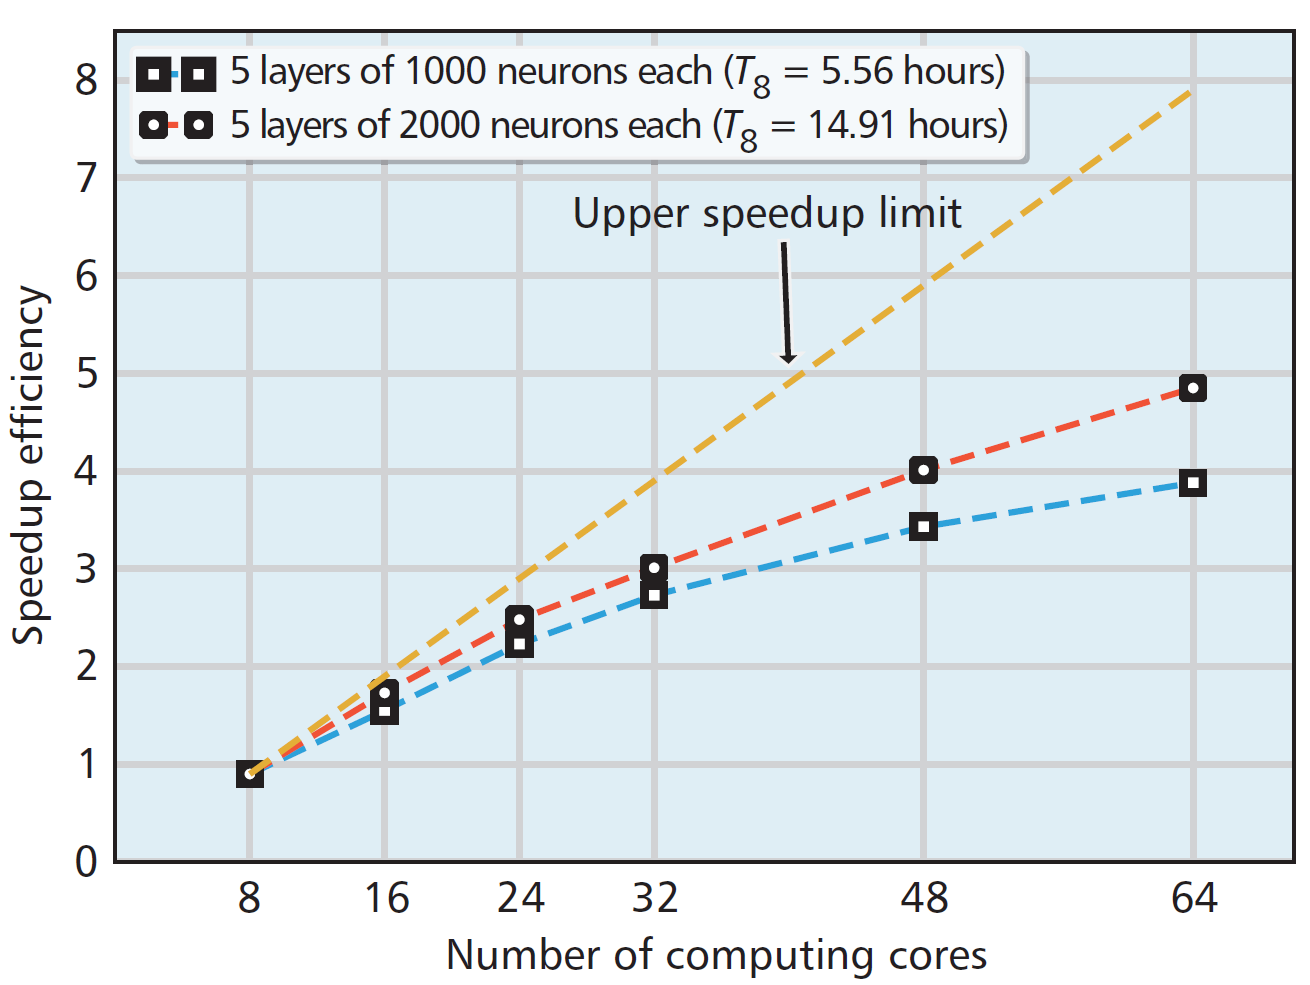
\includegraphics[width=.70\linewidth]{resources/analysis3.png}
        \captionof{figure}{Speedup of learning deep models using Spark-based framework under different computing cores.}
        \label{fig:computingCore}
    \end{figure}
    
\end{frame}

\section{Conclusion}
\begin{frame}{Conclusion}
  \begin{itemize}
      \item{\textit{In this presentation, a scalable Spark-based framework for deep learning in mobile big data was presented.}}
      \item{\textit{The framework enables the tuning of deep models with many hidden layers and millions of parameters on a computing cluster}}
      \item{\textit{The framework has been validated using a large-scale activity recognition system as a case study}}
  \end{itemize}
\end{frame}

\section{Thank you all!  Any Questions?}

\end{document}